\documentclass[12pt]{beamer}

\usepackage{pgfpages}
%\usepackage{handoutWithNotes}


\setbeameroption{show notes on second screen=right}

\setbeamertemplate{note page}{\pagecolor{white!5}\insertnote}\usepackage{palatino}

\begin{document}

\begin{frame}
  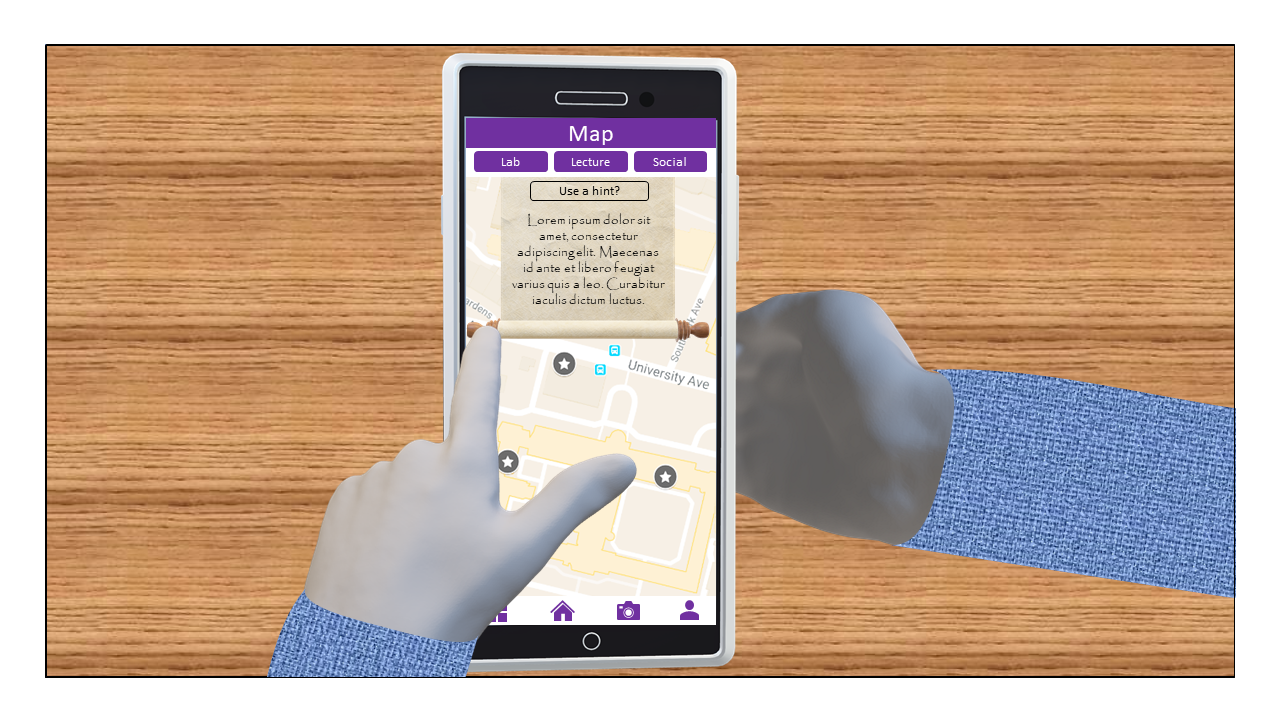
\includegraphics[width=\paperwidth]{./figures/final_storyboards/Slide11.png}
  \note{After completing the personality test, Alan chooses to view the map to discover where there are locations, and to be able to choose his first riddle.
  By tapping the button for one of the three types of location at the top of the screen overlapping the map, he starts that riddle.
  The riddle “unravels” like an ancient roll, and rolls down from the top of the screen to halfway through it, leaving space for Alan to read the riddle clearly and still see the map underneath.
  As the riddle is unravelling, the phone plays a subtle sound effect, similar to that of old paper scroll rolling.
  Once he is done reading the riddle, he swipes up or taps on the riddle and it hides itself by rolling up and disappearing behind the buttons.
  As the riddle is rolling up, the phone plays the scroll sound effect again.
  }
\end{frame}

\begin{frame}
  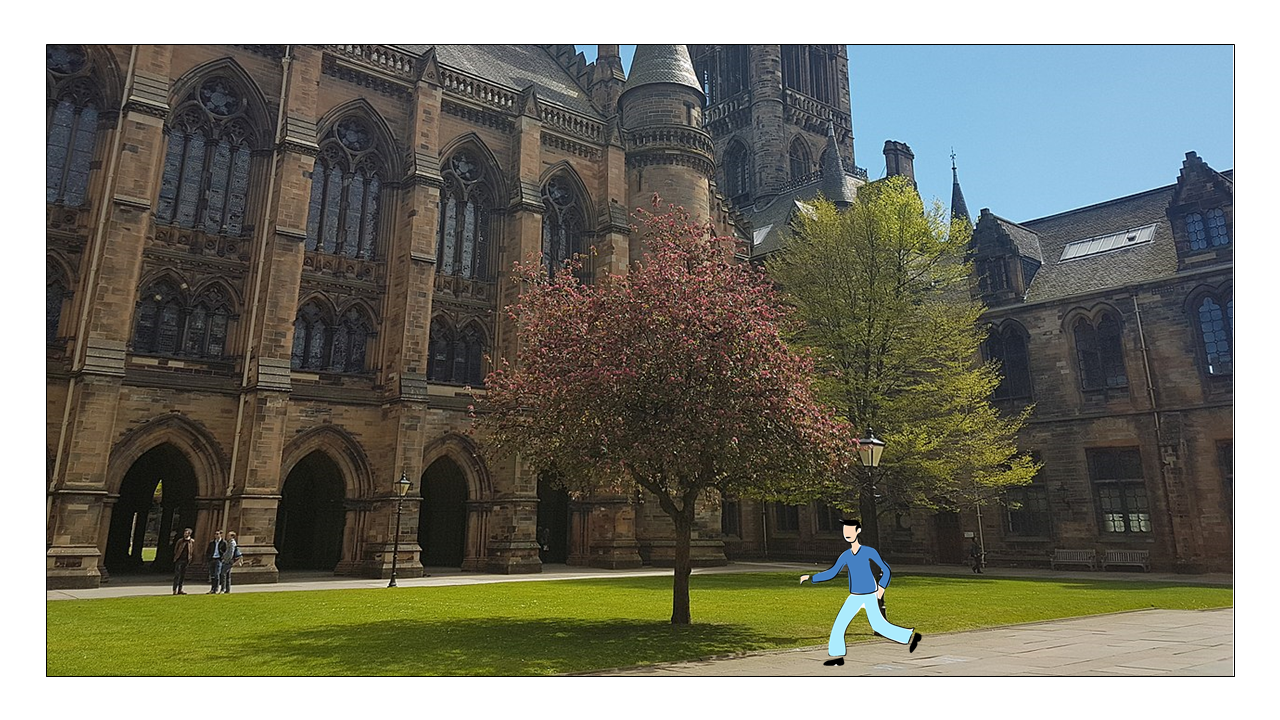
\includegraphics[width=\paperwidth]{./figures/final_storyboards/Slide12.png}
  \note{Alan heads to the building he believes the solution is in.
  He has his phone in his pocket, as he does not need it for navigation.
  He has a choice to take it out to look at the map and find locations, but the app does not show him where the solution of the riddle is or how to get there.
  }
\end{frame}

\begin{frame}
  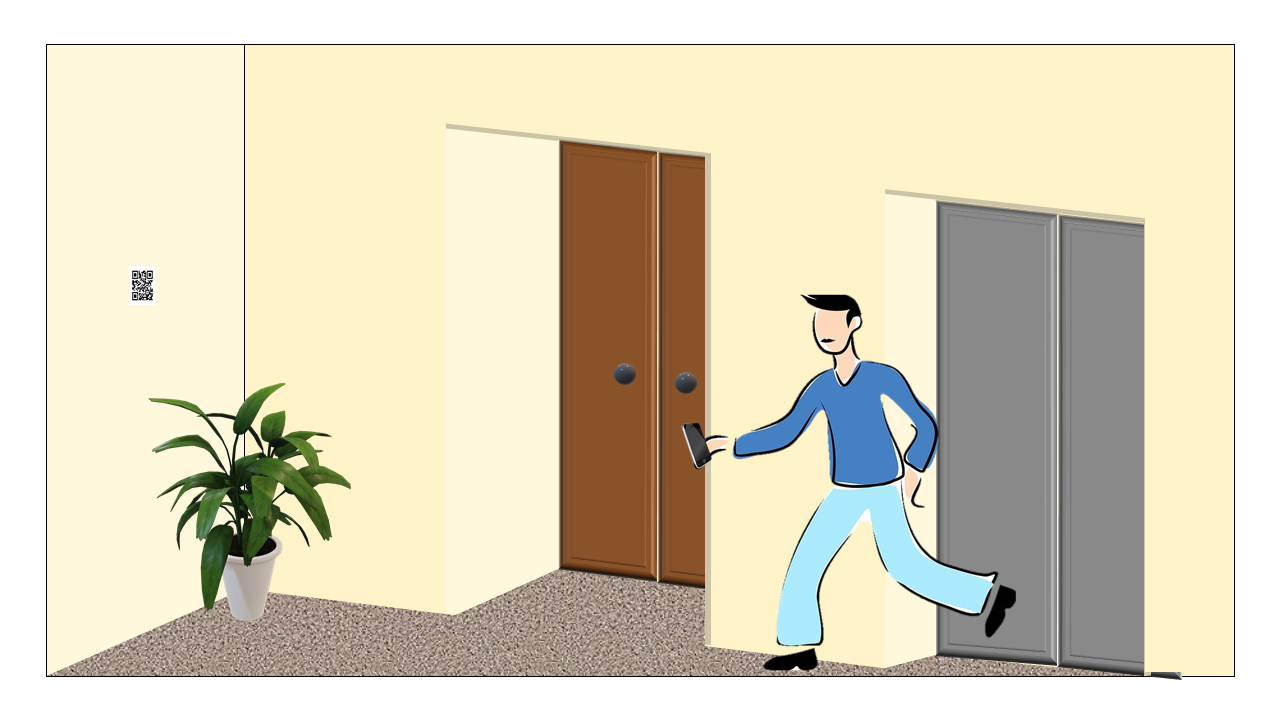
\includegraphics[width=\paperwidth]{./figures/final_storyboards/Slide13.png}
  \note{Alan steps out of the elevator and notices the QR code.
  He is happy that his intuition was correct, and he solved the riddle correctly.
  He proceeds to the code, not blocking other people’s entrance to the lab.
  He takes out his phone from his pocket to open the app and check in at the checkpoint.
  }
\end{frame}

\begin{frame}
  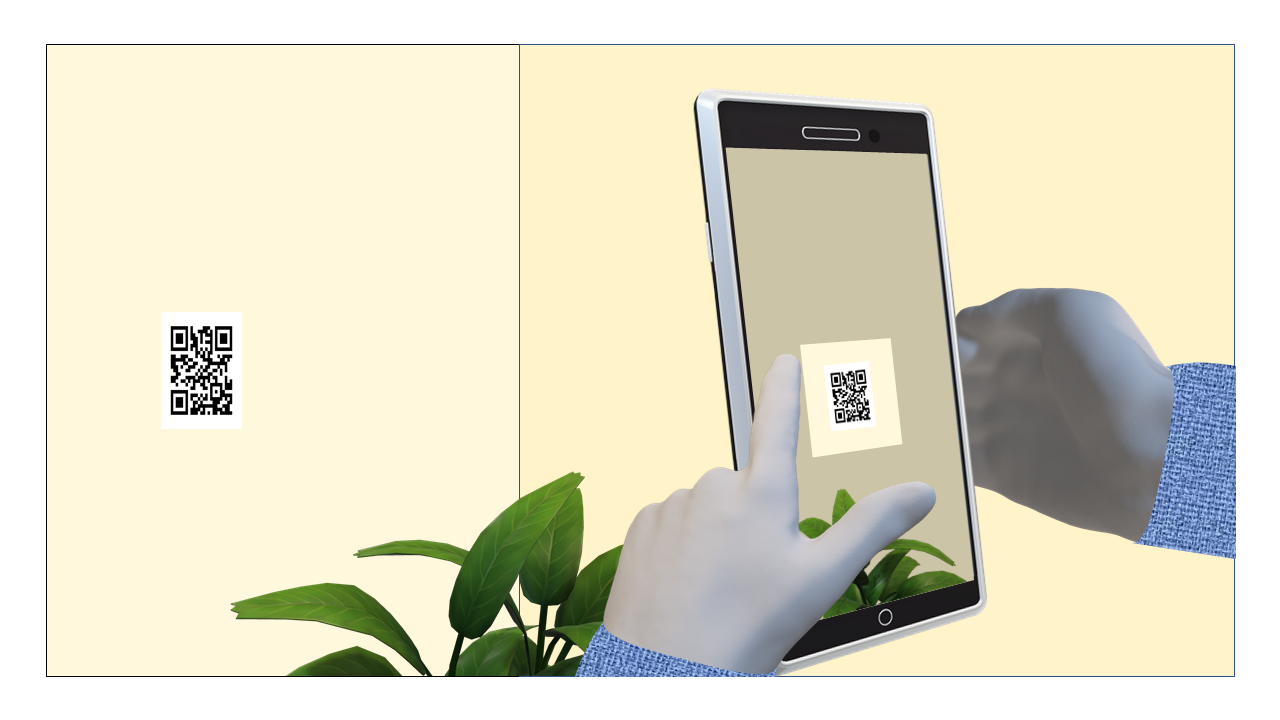
\includegraphics[width=\paperwidth]{./figures/final_storyboards/Slide14.png}
  \note{Alan taps on the camera button at bottom of the screen.
  The phone gives him audio feedback by playing a subtle “pop” sound, similar to that of mobile Operating Systems allocating for keyboard taps.
  The screen quickly changes as the build in camera feature opens in the app.
  The screen shows a bounding box with grey tint on the screen outside the bounding box – this shows Alan that he needs to move the QR code inside the bounding box to scan it.
  When the app registers the code, the phone slightly vibrates once to show Alan it was successfully read.
  }
\end{frame}

\begin{frame}
  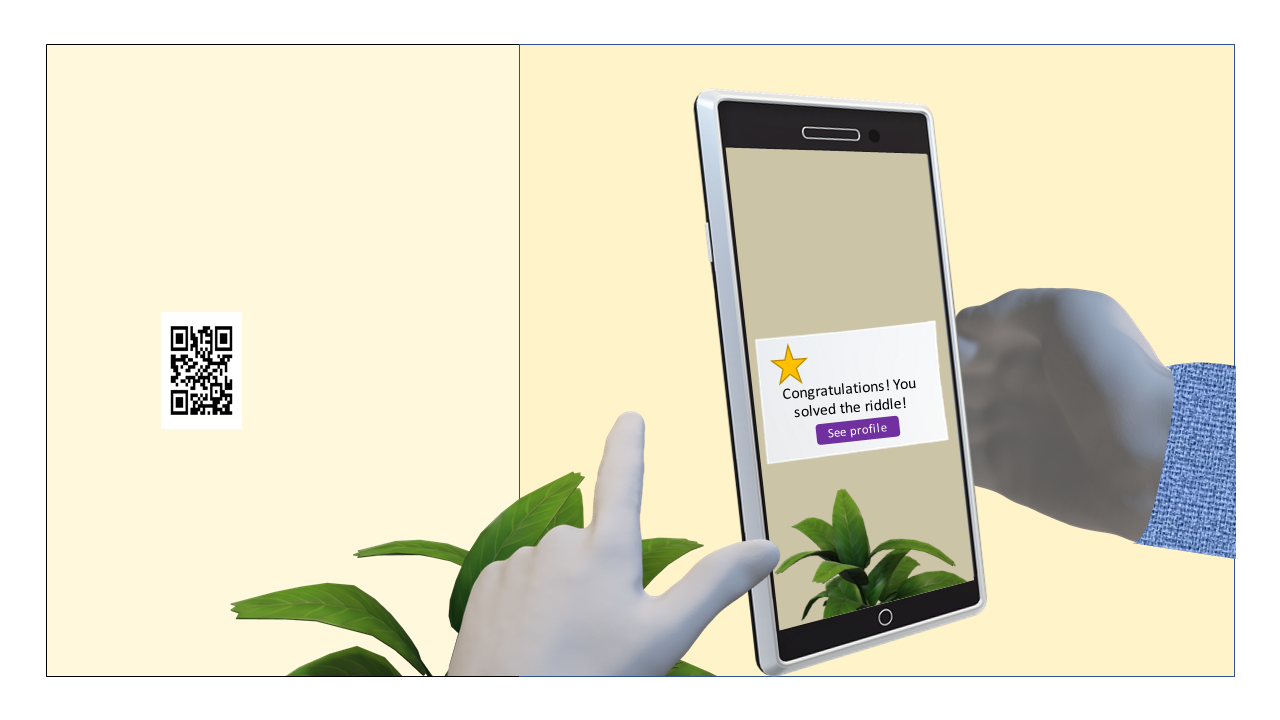
\includegraphics[width=\paperwidth]{./figures/final_storyboards/Slide15.png}
  \note{If the riddle was solved correctly and Alan arrived at the location the riddle told him to, the phone vibrates three times to signal to him he succeeded. At the same time, a small, triumphant sound effect plays to collaborate the physical feedback.
The screen also changes, and a popup tells Alan he scanned the location and the riddle was solved.
The app then presents him with the option to check his profile and view all the XP he’s gained, if he has levelled up, and if he gained any new freebies.
  }
\end{frame}

\begin{frame}
  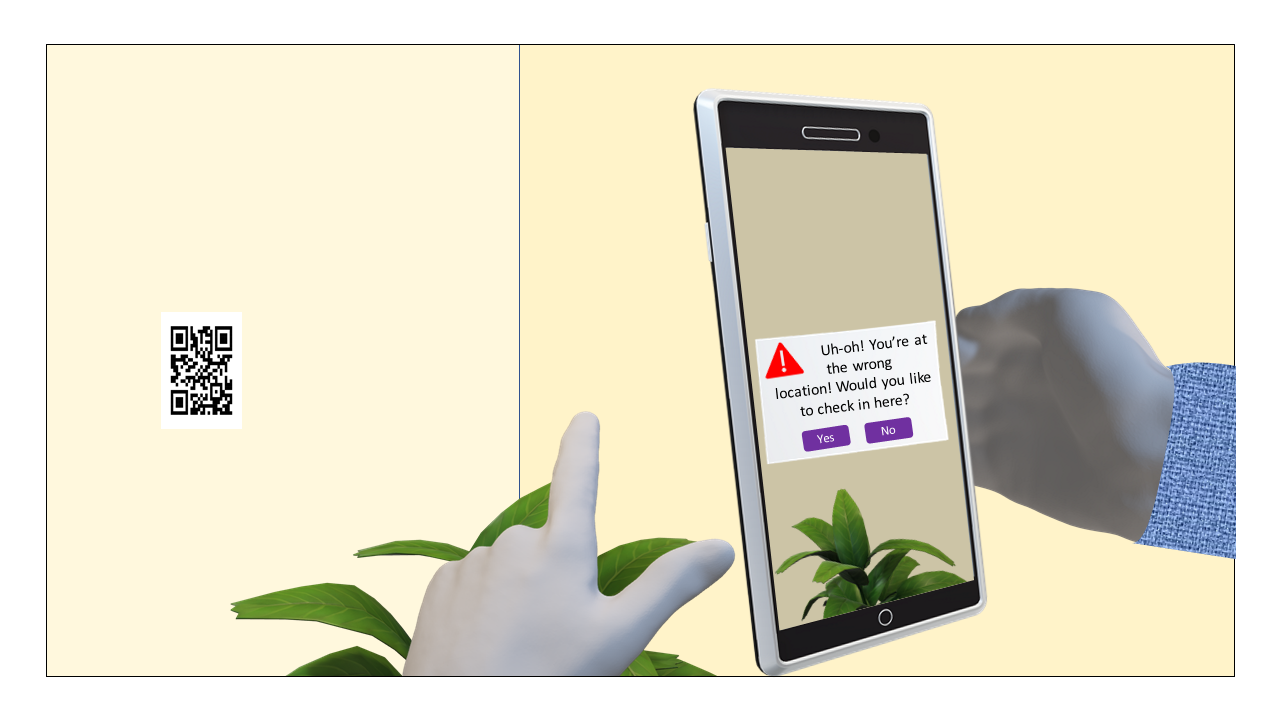
\includegraphics[width=\paperwidth]{./figures/final_storyboards/Slide16.png}
  \note{If the riddle was solved incorrectly and Alan arrived at a location different to what the riddle told him to, the phone vibrates twice to signal to him he got the answer wrong.
The screen also changes, and a popup tells Alan that he is in the wrong location.
The application then presents him with the option to register this location as the wrong answer to the riddle, or to not register the check-in and allow him to try figure out the correct answer.
  }
\end{frame}

\begin{frame}
  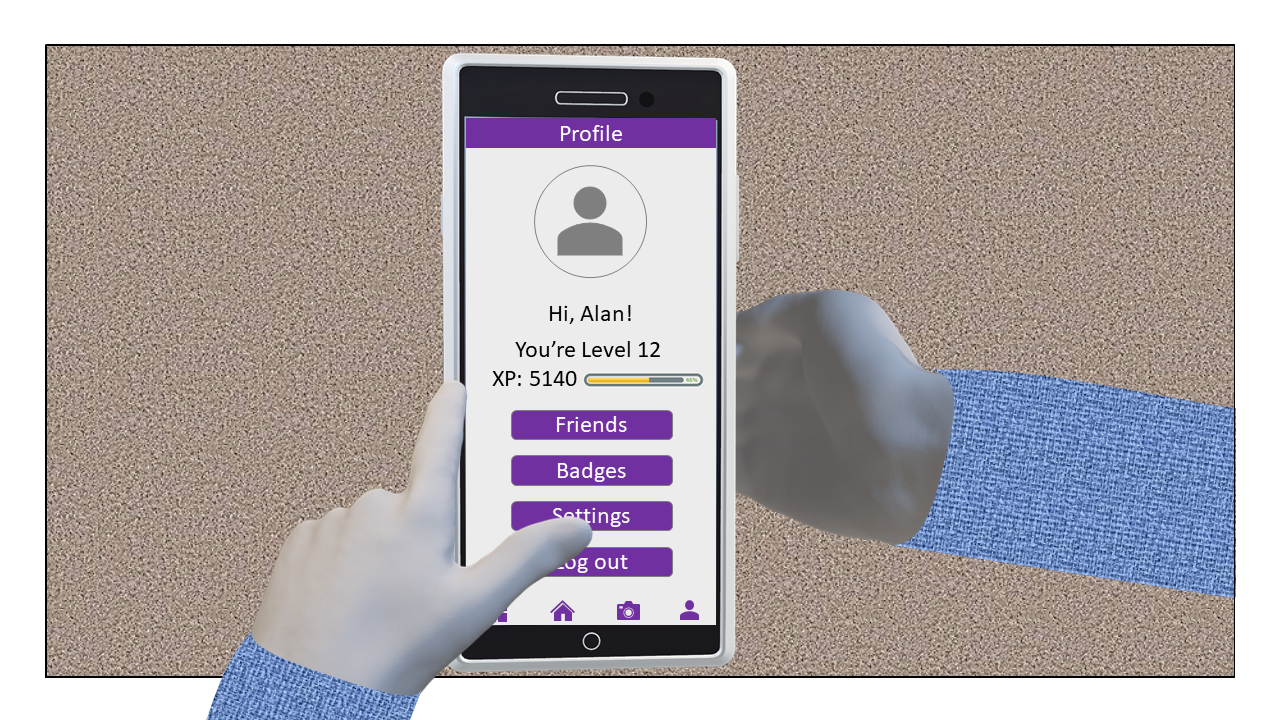
\includegraphics[width=\paperwidth]{./figures/final_storyboards/Slide17.png}
  \note{After having completed a checkpoint, Alan views his in-game progress.
  He does so by tapping on the Profile button at the bottom of the screen.
  With any button press in this screen, the app plays the same “pop” sound effect as on the map menu.
  He views his XP, his list of friends, his in-game level, his badges earned, and can also adjust the app settings or log out if he wants to.
  He is pleased to see he is close to levelling up, and with the new level, he is to gain new freebies.
  }
\end{frame}

\begin{frame}
  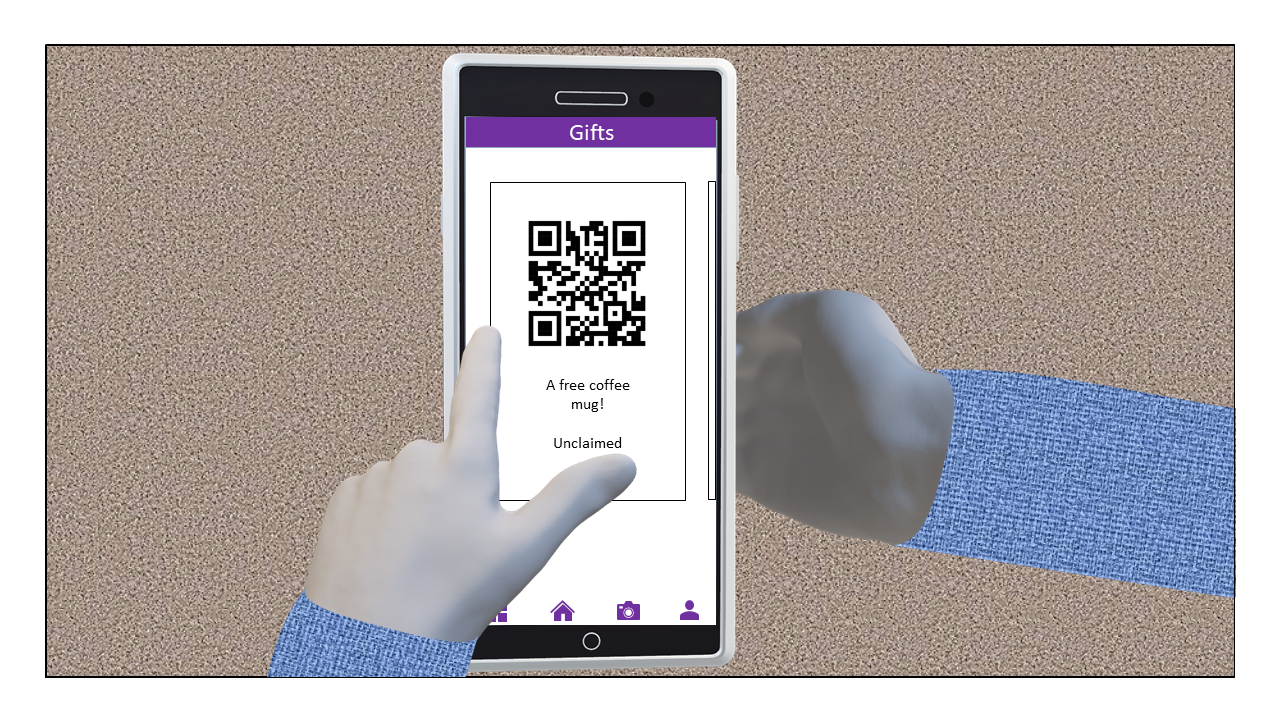
\includegraphics[width=\paperwidth]{./figures/final_storyboards/Slide18.png}
  \note{After having realised that he has gained enough points to qualify for one of the freebies, he views them.
  He does so by tapping on the “Freebies” button at the bottom of the screen.
  When he opens the screen, freebies are contained in smaller item tags, with the next item slightly showing at the right side of the screen.
  This is to signal that Alan can swipe right to see the other freebies.
  When he wants to claim the freebie, he can tap on the freebie item, which blows the image up, and the information contained on the small tab in the list will then fill the screen.
  This is to make it easier too claim the item, by making it easier for the shop assistants to scan the code.
  When the freebie has not been claimed yet, a label states it has been unclaimed. Once he has had a shop assistant scan the code and claimed the item, Alan will see that the item has now changed to be claimed.
  }
\end{frame}

\end{document}